\cleartorightpage
\begin{savequote}[75mm]
``Werken en feesten vormt schoone geesten.''
\qauthor{Johanna Westerdijk}
\end{savequote}

\chapter{Summary}\label{chapter:summary}
\setcounter{figure}{-1}
\setcounter{table}{-1}
\setcounter{section}{-1}
\setcounter{NAT@ctr}{-1}

\begin{figure}[t!]
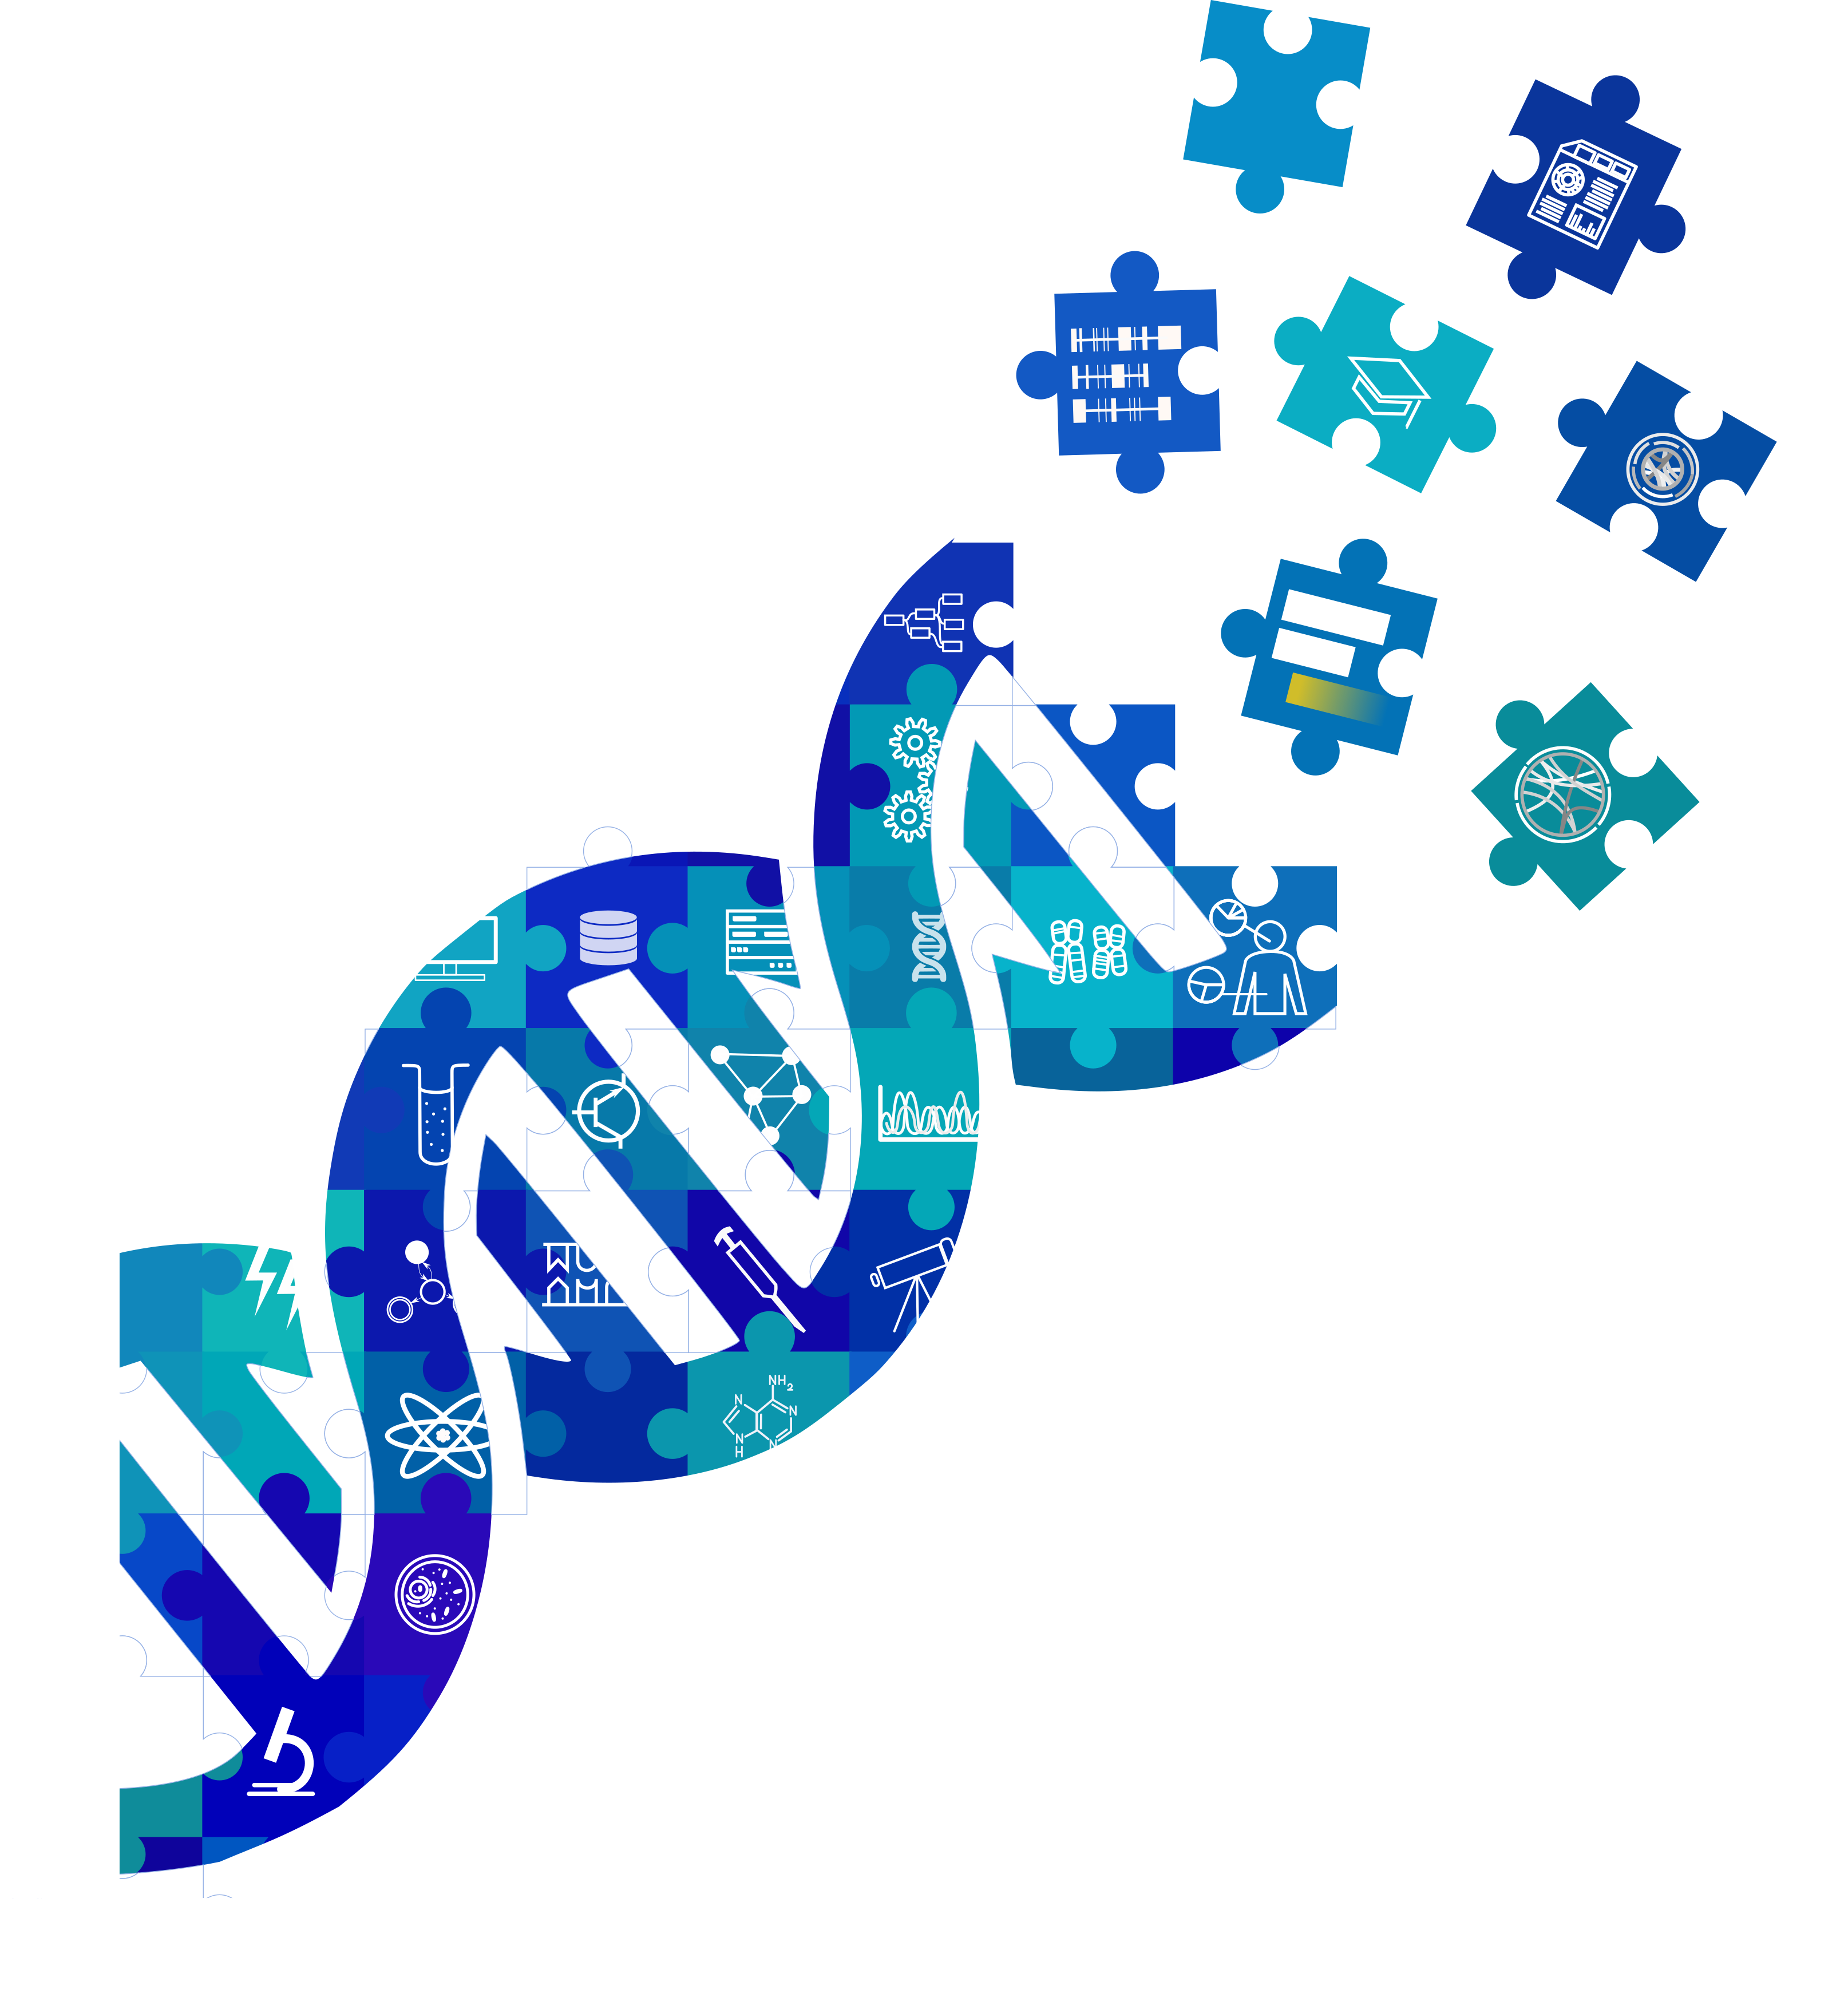
\includegraphics[height=10em]{frontmatter/images/samenvatting.png}
\end{figure}

\begin{enumerate}[label=\color{emc-dark-blue}{\ref{chapter:summary}.\arabic*}]
\itemsep-0.5em
\setcounter{enumi}{-1}
\item English Summary
\item Dutch Summary
\end{enumerate}


\section{Summary}\label{section:summary-en}
\phantomsection\addcontentsline{toc}{section}{Summary}

DNA is often referred to as the \emph{source code of life}; it encodes the proteins that control the functioning of our cells and plays a huge role in our health. The publication of the human reference genome in 2003, combined with sustained technological advances in genome sequencing ever since, have transformed the field biomedical research, and have led to an explosion of the amount of data being generated.
However, scientists typically are not trained in the skills required to manage and analyse these large datasets. Furthermore, bioinformatics tools and workflows tend to be very complex, and often require programming skills to run. As a result, researchers often rely on bioinformaticians to perform the data analyses for them.
This skills gap can lead to the bioinformatics data analysis feeling like a mystical \textit{black box} to the researchers and clinicians tasked with interpreting the data analysis results.
However, a basic understanding of the tools and processes that make up the analysis pipelines is often crucial for an accurate understanding of the analysis results. In this thesis, we aim to shine a light into this black box; to de-mystify bioinformatics, and increase the accessibility of tools and workflows in order to empower researchers and clinician to run their own data analyses.
To this end, we first developed the required technical framework, both for the data analysis itself, and for the training of researchers and clinicians in the use of bioinformatics tools and workflows. We then proceeded to applied this framework and the Open Science methodology to a set of use cases, in prostate cancer analysis and microbiota profiling.

\textbf{Chapter~\ref{introduction}} gives a short introduction to genomics, including a brief history of genome sequencing. It also describes the bioinformatics challenges faced in the analysis of these often large and complex datasets, and provides a set of best-practice guidelines to facilitate accessibility, reproducibility and interoperability of bioinformatics processes. Finally, it provides a short background for each of the use cases, including fusion genes in prostate cancer, and microbiota profiling.

In order to make bioinformatics analyses more accessible to the domain experts, some technical groundwork is required. This is provided in
\textbf{Chapter~\ref{chapter:general}}. Here we introduce the Galaxy platform, a web-based bioinformatics workflow engine that enables scientist to analyse large datasets with nothing more than a web browser.
Once data has been analysed, it must be presented in a comprehensible way to the researchers and clinicians capable of interpreting the results. Efficient visualisation of data is crucial here.
Therefore, as part of this chapter, we have integrated the Circos tool into the Galaxy framework. This tool allows us to plot genome-wide data in a single circular plot. By using Galaxy, this tool becomes accessible to non-bioinformaticians as well.
Finally, we developed iReport, a tool within the Galaxy framework that allows the creation of custom web-reports for results reporting. This tool can combine results from any number of tools, and may be tailored to fit the user's need. Together, these components form the basis for bringing bioinformatics analysis to biomedical researchers and clinicians.

With the technical framework in place, the next important step is the training of the researchers and clinicians in the use of this platform, as well as in the relevant computational an informatics concepts that may impact interpretation of analysis results.
To this end, in \textbf{Chapter~\ref{chapter:training}}, we developed the Galaxy training repository, in close collaboration with the University of Freiburg. This project created a central repository for Galaxy-based training materials. It is a inherently community-driven project, and we put great effort into facilitating contributions from researchers and teachers around the globe.

Next, we applied this process for accessible bioinformatics to a number of use cases. In \textbf{Chapter~\ref{chapter:fusiongenes}} we examined fusion genes in a prostate cancer cell-line. First, we developed iFUSE, a web-based application for the visualisation and exploration of potential fusion genes. This application was used to identify a large number of fusion genes in the VCaP cell-line, and prioritize them on basis of confidence and impact for further confirmation. Furthermore, we determined that one of the arms of chromosome 5 had undergone chromothripsis. This is a shattering of the genome in a single catastrophic event, and the subsequent imprecise stitching back together of the chromosomes by the cell's repair mechanisms. Using the Circos tool we were able to visualize this very effectively.
A second use case within the prostate cancer domain is described in \textbf{Chapter~\ref{chapter:virtualnormal}}. When sequencing tumour samples, typically a sample from healthy tissue of the same patient is also sequenced, in order to distinguish the cancer-specific (somatic) variants from the germline variants. However, such an associated normal sample is not always available. For these cases, we examined the feasibility of using a \emph{virtual normal} instead. This is a set of healthy genomes from healthy, unrelated, genetically diverse individuals. To this end, we first integrated a suite tools for variant analysis and visualisation into Galaxy, and combined them into a workflow.

In addition to these two research-oriented use cases, \textbf{Chapter~\ref{chapter:microbiota}} describes a clinical use case. Here we developed the MYcrobiota platform for diagnostic microbiota profiling using 16S sequencing. This pipeline was developed for use by Streeklab Haarlem as an augmentation to their clinical diagnostic practices when traditional methods do not provide a clear answer.
First, we integrated the full mothur suite of 125+ tools into Galaxy, and then combined them into a workflow. In order to accommodate the specific experimental setup employed by the Streeklab, we additionally developed a set of auxiliary Galaxy tools to supplement the standard analysis pipeline.
These tools, as well as several preexisting Galaxy tools were integrated into an end-to-end workflow, with an iReport at the end for results reporting. This workflow was carefully tested and validated in collaboration with the Streeklab. We also developed Docker images with the full Galaxy setup so that it can be run in-house by the Streeklab.

For each of these use cases, we adhered to the bioinformatics best-practices and Open Science principles outlined in the introduction, and all the code is freely available in GitHub. Training materials have also been developed in order to aid not only our own researchers and clinicians in the use of the tools and workflows we developed, but also others around the world. All these training materials have deposited in the Galaxy training repository described in Chapter~\ref{chapter:training}.


\section{Samenvatting}
\phantomsection\addcontentsline{toc}{section}{Samenvatting}

DNA word vaak beschouwd als de \emph{broncode van het leven}; het encodeert
de eiwitten die onze celprocessen beinvloeden, en speelt een belangrijke rol in onze gezondheid.
De publicatie van het humane referentie genoom in 2003, in combinatie met continue technologische vooruitgangen sindsdien, hebben het veld van biomedisch onderzoek volkomen getransformeerd, en hebben geresulteerd in een explosie van de hoeveelheid data die gegenereerd wordt in de biomedische wetenschappen.

Wetenschappers worden echter meestal niet opgeleid in de benodigde vaardigheden om deze efficient om te gaan met deze grote hoeveelheden complexe datasets en ze te analyseren.
Verder zijn bioinformatica tools en pijplijnen vaak erg complex, en zijn programmeervaardigheden meestal benodigd om ze te kunnen gebruiken. Hierdoor onstaat de situatie waarin onderzoekers vaak afhankelijk zijn van gespecialiseerde bioinformatici om hun analyses uit te voeren.
Door deze vaardigheidskloof kan bioinformatica vaak aanvoelen als een \emph{black box} voor de onderzoekers en clinici die de resultaten van deze analyse moeten interpreteren.
Desalniettemin is een basiskennis van de achterliggende computationele concepten vaak essentieel voor de accurate interpretatie van de resultaten.
In dit proefschrift trachtten wij de bioinformatische \emph{black box} te illumineren, en de tools en pijplijnen toegankelijk te maken voor onderzoekers en clinici, zodat ze hun eigen data analyses weer uit kunnen voeren, zonder afhankelijk te zijn van tussenkomst van een bioinformaticus.

Hiervoor hebben we eerst de technische grondslag ontwikkeld, zowel voor het uitvoeren van de data analyses, alsmede het opleiden van onderzoekers en clinici in het gebruik ervan. Vervolgens hebben we dit technische framework toegepast via een set van wetenschappelijke casussen, in het gebied van prostaatkanker en micribiota analyse.

\textbf{Hoofdstuk~\ref{introduction}} geeft een korte algemene introductie tot genomics, waaronder een korte geschiedenis van sequencing technologieen.
Hierbij worden ook de uitdagingen beschreven die we tegenkomen in de bioinformatica bij het analyseren van de resulterende grote en complexe datasets, en geven we een set richtlijnen voor het faciliteren van toegankelijke, reproduceerbare en interoperabele data analyse.
Tot slot wordt hier een korte achtergrond gegeven voor ieder van de casussen.

\textbf{Hoofdstuk~\ref{chapter:general}} beschrijft de technische grondslag die we ontwikkeld hebben om de bioinformatica meer toegankelijk te maken voor de wetenschappelijke experts die de data genereren en de resultaten zullen interpreteren.
Hier introduceren we allereerst Galaxy, een gebruiksvriendelijk data analyse platform waarmee wetenschappers makkelijk hun datasets kunnen analyseren met enkel een web browser. Na het analyseren van de data moeten de resultaten op een gestructureerde en overzichtelijke manier gepresenteerd worden aan de gebruiker. Visualizatie is hierbij cruciaal.
Daarom hebben we als tweede deel van dit hoofdstuk de Circos tool in Galaxy geintegreerd. Circos is een krachtige tool waarmee we genoom-wijde data efficient in een circulair plot kunnen weergeven.
Normaalgesproken vergt deze tool gespecialiseerde kennis van bioinformatica, maar door deze binnen Galaxy beschikbaar te maken kan de tool ook gebruikt worden zonder deze technische kennis.
Tot slot beschrijft dit hoofdstuk de iReport tool, waarmee gebruikers zelf web reports kunnen configureren binnen Galaxy om de resultaten van hun analyses weer te geven, wat precies afgestemd kan woorden op hun behoeften.
Samen zorgen deze 3 componenten ervoor dat NGS analyses toegankelijk worden voor biomedische onderzoekers en clinici.

Met de technische grondslag gelegd, is de volgende belangrijke stap het opleiden van onderzoekers
en clinici om hiermee om te gaan, zowel als de benodigde basiskennis op te doen over de achterliggende computationele concepten die een effect kunnen hebben op de interpretatie van de resultaten.
In \textbf{Hoofdstuk~\ref{chapter:training}} hebben we een de Galaxy Training Repository ontwikkeld, in nauwe samenwerking met de Universiteit van Freiburg.
In dit project hebben we een centrale repository ontwikkeld voor het verzamelen en onderhouden van wetenschappelijke training materialen die begruik maken van het Galaxy platform.
Door de grootschalige aard van dit project, is het zo opgezet dat gebruikersgemeenschap rond Galaxy het project samen draaiend kan houden, en gebruik gemaakt kan worden van de gecombineerde expertise van wetenschappers en opleiders over de hele wereld.

Vervolgens hebben we deze aanpak toegepast op een aantal casussen. In \textbf{Hoofdstuk~\ref{chapter:fusiongenes}} hebben we fusie genen in een prostaatkanker cellijn onderzocht. Hiervoor hebben we eerst een applicatie ontwikkeld (\emph{iFUSE}) voor het visualiseren van structurele varianten en het identificeren van fusiegen kandidaten.
Door gebruik van deze applicatie, in combinatie met de Circos tool, waren we in staat een groot aantal potentiële fusie genen te identificeren in de VCaP cellijn, en hebben we deze bevindingen in het lab kunnen bevestigen.
Verder hebben we zo ook kunnen vaststellen dat de q arm van chromosoom 5 \emph{chromothripsis} vertoonde, een phenomeen waarbij een deel van het genoom verbrijzeld wordt, waarna het genetische materiaal vervolgens op inaccurate wijze weer aan elkaar geplakt wordt door de reparatiemechanismen van de cel.

Een tweede casus binnen het prostaat kanker domein beschrijven we in \textbf{Hoofdstuk~\ref{chapter:virtualnormal}}. Wanneer we een tumor sequencen, wordt er normaal gesproken meestal ook gezond weefsel van dezelfde patient gesequenced.
Hierdoor kunnen we de tumorcellen vergelijken met gezonde cellen, om zodoende de kanker-specifieke varianten te onderscheiden van de germline cellen.
Echter, zo'n geassocieerd normaal sample is niet altijd beschikbaar.
In zulke gevallen wilden we achterhalen of deze aanpak gesimuleerd kon worden door het gebruiken van een grote set van monsters afkomstig van gezonde, ongerelateerde, ethnisch diverse individuelen.
Hiervoor hebben we eerst een set analyse tools geidentificeerd en ontwikkeld, en deze in Galaxy beschikbaar gemaakt, en ze gecombineerd tot een pijplijn.

Naast deze twee onderzoeks georienteerde toepassingen, beschrijven we in \textbf{Hoofdstuk~\ref{chapter:microbiota}} een derde, clinisch georienteerde casus. Hier hebben we het MYcrobiota platform ontwikkeld voor de profilering van microbiota via 16S rRNA sequencing voor gebruik binnen de diagnostiek.
Deze applicatie is ontwikkeld in samenwerking met het Streeklab Haarlem, als aanvulling op hun traditionele diagnostiek, wanneer de resultaten daarvan geen uitsluitsel geven.

Hiervoor hebben we eerst de complete mothur toolkit van 125+ tools in Galaxy geintegreerd, en een workflow gemaakt die precies afgestemd is op de exacte experimentele setup van het Streeklab.
Hiervoor moesten ook een aantal nieuwe tools gescherven worden als aanvulling op de standaard analyse procedure.
Deze tools, in combinatie met reeds bestaande Galaxy tools, hebben we samengevoegd tot een pijplijn, met een iReport aan het eind voor het presenteren van de resultaten aan de clinici.
Deze pijplijn is grondig getest en gevalideerd in samenwerking met de experts op het Streeklab, alvorens in gebruik genomen te worden.
Om het mogelijk te maken om MYcrobiota binnenshuis te draaien op het Streeklab, hebben we Docker images ontwikkeld met alle benodigdheden om de applicatie gemakkelijk overal te kunnen draaien.

Voor al deze toepassing hebben we ons gehouden aan de richtlijnen die we hebben beschreven in de introductie, en alle code is compleet open en voor iedereen vrij te gebruiken. Ook hebben we voor iedere casus training materialen ontwikkeld, en ondergebracht in de Galaxy training repository beschreven in \textbf{Hoofdstuk~\ref{chapter:training}}, waardoor ze niet alleen beschikbaar zijn voor onze eigen onderzoekers en clinici, maar voor de wereldwijde gebruikersgemeenschap.


